\section{Question 4\label{section:ex4}}


\colorlet{droplet color}{blue!50!cyan!80}
\tikzset{%
  raindrop/.pic={
    code={\tikzset{scale=1/10}
 \shade [shading=droplet]
 (0,0)  .. controls ++(0,-1) and ++(0,1) .. (1,-2)
 arc (360:180:1)
 .. controls ++(0,1) and ++(0,-1) .. (0,0) -- cycle;
  }}}

\begin{figure}[H]
\begin{center}
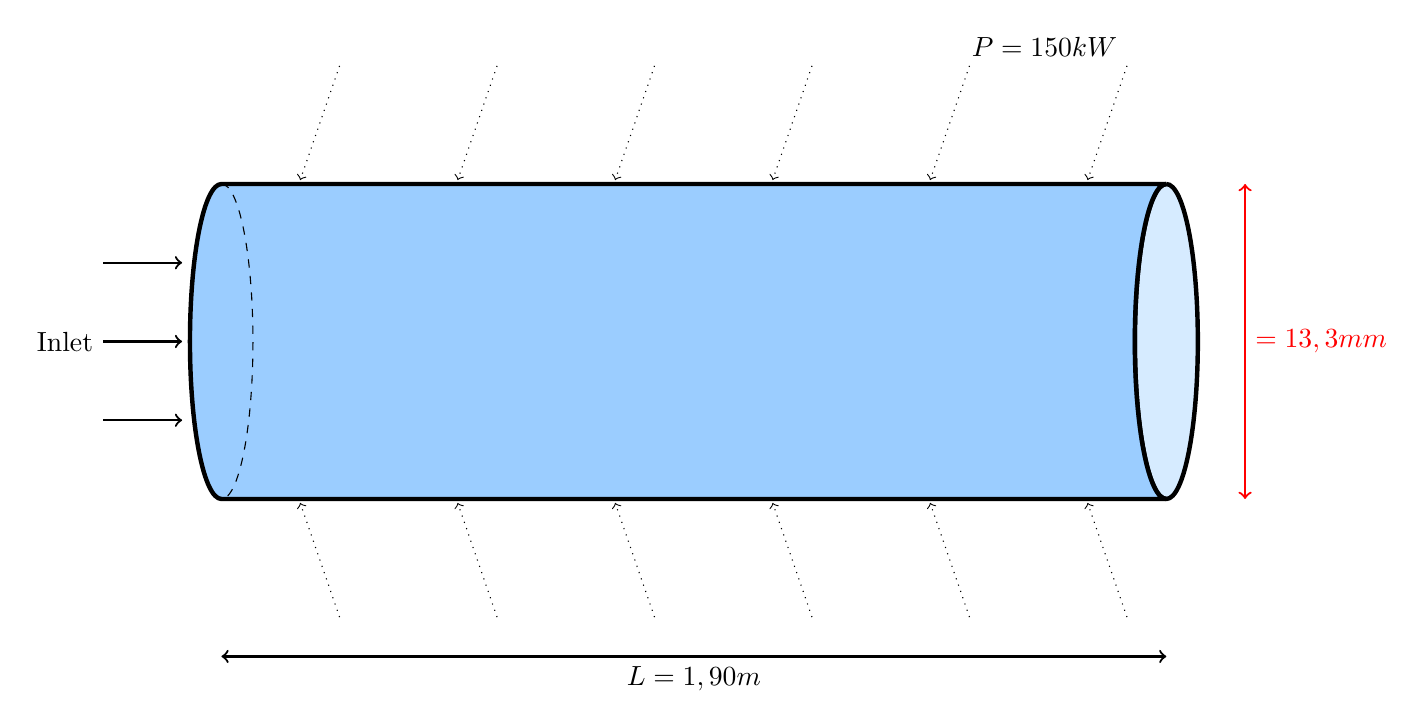
\begin{tikzpicture}[line join=round,rotate=270]
\filldraw[draw=black,ultra thick,fill=droplet color!20]
 (0,12) arc[x radius=2, y radius=0.4, start angle=180, end angle=0]
 (4,12) arc[x radius=2, y radius=0.4, start angle=0, end angle=-180];
\filldraw[ultra thick,fill=droplet color!70,opacity=1,fill opacity=0.7]
  (0,12) -- 
  (0,0) 
  arc[x radius=2, y radius=0.4, start angle=-180, end angle=0] --
   (4,12)
  arc[x radius=2, y radius=0.4, start angle=0, end angle=-180];
\draw[dashed] 
  (0,0) arc[x radius=2, y radius=0.4, start angle=180, end angle=0];

%\draw[red,<->, thick] (0,9) -- (1,9)node[right] {$R$}-- (2,9);
\draw[black,->,dotted] (-1.5,1.5) -- (-0.05,1);
\draw[black,->,dotted] (-1.5,3.5) -- (-0.05,3);
\draw[black,->,dotted] (-1.5,5.5) -- (-0.05,5);
\draw[black,->,dotted] (-1.5,7.5) -- (-0.05,7);
\draw[black,->,dotted] (-1.5,9.5) -- (-0.05,9);
\draw[black,->,dotted] (-1.5,11.5)node[above left]{$P = 150 \si{kW}$} -- (-0.05,11);

\draw[black,->,dotted] (5.5,1.5) -- (4.05,1);
\draw[black,->,dotted] (5.5,3.5) -- (4.05,3);
\draw[black,->,dotted] (5.5,5.5) -- (4.05,5);
\draw[black,->,dotted] (5.5,7.5) -- (4.05,7);
\draw[black,->,dotted] (5.5,9.5) -- (4.05,9);
\draw[black,->,dotted] (5.5,11.5) -- (4.05,11);

\draw[black,->,thick] (1,-1.5) -- (1,-0.5);
\draw[black,->,thick] (2,-1.5)node[left]{Inlet} -- (2,-0.5);
\draw[black,->,thick] (3,-1.5) -- (3,-0.5);

\draw [thick,red] [<->] (0,13) --++(2,0) node [right] {$\varnothing = 13,3 \si{mm}$} --++(2,0);
\draw [thick] [<->] (6,0) --++(0,6) node [below] {$L=1,90 \si{m} $}--++(0,6);
%\draw [thick] [->] (1,10.5) --++(-0.5,-0.4) node [below left]
%{$\vec{e_{\theta}}$};
%\draw[dashed] (2,9.9)--(1.5,10.2)node [right]{$r$}-- (1,10.5);


%\draw[black,dotted, thick] (0,2) -- (4,2);
%\draw[black,dotted, thick] (0, 2) .. controls(1,4) and (3,4) .. (4, 2);
%\draw[black,->, thick] (1,2) -- (1,3.1);
%\draw[black,->, thick] (3,2) -- (3,3.1);
%\draw[black,->, thick] (2,2) -- (2,3)node[below] {$\vec{u}$} -- (2,3.5);
%\draw[black,->, thick]    (2.5,3) -- (2.5,4)node[below] {$\dot{Q}_G = 0,002$ \si{m^3/s}} -- (2.5,5);
\end{tikzpicture}

\caption{Schéma de la conduite pour étudier la chute de pression}
    \label{fig:ConfigExo4}
    \end{center}
\end{figure}

Dans cet exercice, nous travaillons avec une conduite chauffée uniformément par une puissance $P = 150 \si{kW}$ comme représentée sur la fig. \ref{fig:ConfigExo4}. Les paramètres à l'entrée de la conduite (noté Inlet sur le schéma) sont donnés comme :

\begin{equation}
    \left\{
    \begin{array}{r c l l}
    P &=& 30 & \si{bar} \\
    T_{SR} &=& 10 & \si{K}\\
    \dot{m} &=& 0.42 &\si{kg/s}
    \end{array}
    \right.
\end{equation}
\\
On rappelle les hypothèses utilisés dans ce problème :
\begin{itemize}
    \item \textbf{H1} : L'écoulement est incompressible.
    \item \textbf{H2} : La perte de pression par accélération dans la région non bouillante est négligeable.
     \item \textbf{H3} : La perte de pression totale est négligeable par rapport à la pression de l'écoulement.
\end{itemize}
\vspace{12pt}
\par
\subsection{Titre thernodynamique nul - $x$}
Comme il y a une température de sous-refroidissement $T_{SR}$ en entrée, la température de saturation de l'eau à 30 \si{bar} (qui est égale à 233,7\degre C) n'est atteinte que plus loin dans la conduite. On cherche donc la distance qu'il faut pour réchauffer l'écoulement de 10 \si{K}, qui correspond à l'endroit où le titre thermodynamique est nul.
On peut écrire :
\begin{equation}
    \dot{Q}_{sat} = \dot{m} Cp \Delta T
\end{equation}
Le terme $Cp$ pouvant être pris pour une pression de 30 \si{bar}, il vaut alors 4715,9 \si{kJ/kg K}. On a trouve alors que la puissance nécessaire est de :
\begin{equation}
    P_{sat} = 19.8 \si{kW}
\end{equation}
Comme on considère que la conduite est chauffée uniformément, le rapport entre puissance nécessaire pour arriver à saturation et puissance totale thermique ajoutée $P_{th}$ est égale au rapport entre $L_{sat}$ et longueur totale chauffée $L_c$. on a alors :
\begin{equation}
\boxed{
    L_{sat}= \frac{ P_{sat}\times L_c}{P_{th}} = \frac{19.8 \times 1,9}{150} = 0.25~\si{m} 
    }
\end{equation}
\subsection{Titre thermodynamique en sortie - $x_s$}
Nous pouvons donc maintenant nous concentrer sur l'obtention du titre en sortie de la conduite.\\
La conservation de l'énergie nous donne la forme suivante pour le titre :
\begin{equation}
    x_s = \frac{4}{G}\frac{1}{D}\frac{q''}{h_{lv,sat}}L
\end{equation}
Cette forme est valable à partir du moment où le titre est nul. Dans notre cas, la conduite ne fait donc plus L = 1.9 \si{m} mais il faut lui enlever la région non-bouillante qui fait 0.25 \si{m}.\\ \par
Définissons maintenant les termes que nous avons besoin pour cette équation. Commençons par les surfaces, il y a la surface de la paroi et la section de la conduite qui donnent respectivement :
\begin{equation}
    S_{par} = L_c \times \pi D = \num{0.0794}~\si{m^2}
\end{equation}

\begin{equation}
    S_{con} = \frac{\pi D^2}{4} = \num{1.3894e-4}~\si{m^2}
\end{equation}
On peut ainsi définir le flux massique $G$ :
\begin{equation}
    G = \frac{\dot{m}}{S_{con}} = \num{3023.13} ~\si{kg/m^2s}
\end{equation}
Et $q''$ le flux de chaleur sur la paroi :
\begin{equation}
    q'' = \frac{P}{S_{par}} = \num{1889,5} ~\si{kW/m^2}
\end{equation}

Enfin le dernier terme nécessaire est $h_{lv,sat}$ qui est la différence entre l'enthalpie à saturation du gaz et du liquide :
\begin{equation}
    h_{lv,sat} = h_{v,sat} - h_{l,sat} = 2803 -1007,7 = 1795,3 ~\si{kJ/kg}
\end{equation}
Les valeurs proviennent des tables de saturation de l'eau à une pression de 30 \si{bar}.\\
On a alors : 
\begin{equation}\boxed{
    x_s = \frac{4}{G}\frac{1}{D}\frac{q''}{h_{lv,sat}} \left(L_c - L_{sat}\right) = 0,173
    }
\end{equation}
\subsection{Perte de pression totale - $\Delta P$}

On peut désormais s'intéresser à la perte de pression dans la conduite qui est de la forme : 
\begin{equation}
\begin{array}{c}
-\Delta P=\frac{1}{2} f \frac{G^{2}}{\rho_{l}} \frac{L}{D} \overbrace{\left[\frac{1}{x_{e}} \int_{0}^{x_{e}} \phi_{l_{0}}^{2} d x\right]}^{\text{Multiplicateur diphasique}}+\frac{G^{2}}{\rho_{l}}\overbrace{\left[\frac{x_{e}^{2}}{\varepsilon_{e}} \frac{\rho_{l}}{\rho_{v}}+\frac{\left(1-x_{e}\right)^{2}}{\left(1-\varepsilon_{e}\right)}-1\right]}^{\Delta P\text{ par accélération}} \\
+\underbrace{\cancel{\frac{L}{x_{e}} g \int_{0}^{x_{e}}\left[\rho_{v} \varepsilon+\rho_{l}(1-\varepsilon)\right] d x}}_{\text{Conduite horizontale $g=0$}}
\end{array}
\end{equation}

Les termes du \og Multiplicateur diphasique \fg{} et \og Perte de pression par accélération \fg{} sont obtenus par lecture dans des abaques. On peut alors, avec le titre en sortie $x_s=17,3\%$ et $P = 30 ~ \si{bar}$ , en déduire :
\begin{equation}
    \left\{
    \begin{array}{r c l}
    \left[\frac{1}{x_{e}} \int_{0}^{x_{e}} \phi_{l_{0}}^{2} d x\right] &=& 8 \\[2ex]
    \left[\frac{x_{e}^{2}}{\varepsilon_{e}} \frac{\rho_{l}}{\rho_{v}}+\frac{\left(1-x_{e}\right)^{2}}{\left(1-\varepsilon_{e}\right)}-1\right] &=& 4 \\
    \end{array}
    \right.    
\end{equation}
Le terme  noté $f$, correspond au facteur de frottement monophasique, défini comme :
\begin{equation}
    f=0.316\left[\text{Re}_L \right]^{-0.25} = 0.316\left[\frac{(1-x) G D}{\mu_l} \right]^{-0.25}
\end{equation}
%La vitesse moyenne de la phase liquide de l'écoulement se détermine avec le %débit massique :
%\begin{equation}
%    u_l = \frac{\dot{m}}{\rho_l}\frac{1}{S_{con}} = 3.67~ \si{m/s}
%\end{equation}
Et en utilisant les valeurs :
\begin{equation}
    \left\{
    \begin{array}{r c l l}
%    \rho_l &=& 823.1 &\si{kg/m^3}\\
    x &=& 0.173 & \\
    \mu_l &=& \num{116,4e-6} &\si{Pa.s}
    \end{array}
    \right.    
\end{equation}
Nous obtenons, $\text{Re}_L = \num{287493,7}$ soit $f = \num{0,0136}$\\

En injectant le tout dans l'équation de la perte de pression on obtient :
\begin{equation}
    \boxed{
    -\Delta P = \num{130709} ~\si{Pa} = 1.31 ~\si{bar}
    }
\end{equation}